\documentclass[10pt,twocolumn]{article}

\usepackage[utf8]{inputenc}
\usepackage[T1]{fontenc}
\usepackage{lmodern}
\usepackage{microtype}
\usepackage[margin=0.72in,top=0.78in,bottom=0.82in]{geometry}
\usepackage{amsmath,amssymb,amsthm}
\usepackage{booktabs}
\usepackage{array}
\usepackage{xcolor}
\usepackage{tikz}
\usepackage{listings}
\usepackage[colorlinks=true,linkcolor=blue!55!black,citecolor=blue!55!black,urlcolor=blue!60!black]{hyperref}

\definecolor{brass}{RGB}{138,103,38}
\definecolor{ink}{RGB}{29,27,24}
\definecolor{codebg}{RGB}{246,245,241}
\definecolor{rulecol}{RGB}{210,205,196}

\lstset{
  basicstyle=\ttfamily\scriptsize,
  backgroundcolor=\color{codebg},
  frame=single,
  rulecolor=\color{rulecol},
  breaklines=true,
  columns=fullflexible,
  keepspaces=true,
  aboveskip=4pt,
  belowskip=4pt
}

\newtheorem{theorem}{Theorem}
\newtheorem{proposition}{Proposition}
\newtheorem{lemma}{Lemma}
\newtheorem{corollary}{Corollary}
\theoremstyle{definition}
\newtheorem{definition}{Definition}

\setlength{\columnsep}{0.24in}

\title{\vspace{-1.0em}\textbf{Scaling Cyclic Multi-Language Quines to 284 Steps and 273 Distinct Languages:\\[0.25em]
\large Affine Escape Dynamics, Piecewise-Contractive Corridors, and Formal Closure Verification}}

\author{
  \textbf{ExaCortex Research} \\
  \small Drawn With Code Studio $\cdot$ \texttt{hello@exacortex.net} \\
  \small Repository \& Proofs: \url{https://github.com/exacortex/quine-relay-284} $\cdot$ Web: \url{https://exacortex.net/record.html}
}

\date{\small November 18, 2026}

\begin{document}
\maketitle

\begin{abstract}
\noindent
A \emph{cyclic multi-language quine} (or \emph{quine relay}) is a closed sequence of programs $P_1, P_2, \dots, P_n$ in distinct programming languages such that executing $P_k$ on its native compiler or interpreter emits the exact source text $P_{k+1}$, with $P_{n+1} \equiv P_1$ byte-for-byte. While Yusuke Endoh's celebrated 128-step Uroboros relay stood as the public high-water mark from 2018 to 2026, naive attempts to double $n$ encounter coupled exponential blowups from nested string escaping alongside hard 16-bit, 24-bit, and heap ceilings in real-world toolchains.

We present \textbf{Quine Relay 284}, a verified 284-step closed loop spanning \textbf{273 distinct Tier-1 programming languages} seeded from a single 42,680-byte Ruby file (\texttt{QR.rb}, SHA-256 \texttt{9ce6dbe3\dots eb509a}). First, we model nested C/POSIX string escaping on the state vector $(B, S, Q) \in \mathbb{N}^3$ (bytes, backslashes, double-quotes) and discover two exact invariants: an eigenvalue-2 functional $\Phi(S, Q) = S + Q + 2$ satisfying $\Phi_k = 2^k \Phi_0$, and a quote-independent byte--backslash conservation law $B_k - S_k = B_0 - S_0 + k w_0$ that predicts empirical payload sizes across multi-step compiler ladders to the exact single byte. Second, we prove a zero-residual delimiter-reset identity showing that replacing an escaping base step with a zero-backslash delimiter parser eliminates $(2^{k+1} - 1)(S_0 + Q_0)$ bytes ($>170\text{ MB}$ across 13 layers). Third, combining telescoping ratio conservation ($\prod_{k=1}^n r_k = 1$), adjacent-swap front-loading, self-reading $O(1)$-AST comment decoders, 3-digit base-78 LZ78 coding ($78^3 = 474{,}552$), and interleaved Re-Pair assembly compression keeps 8-bit 6502 and Z80 machine-code ROMs under 46 KB and caps peak intermediate output below 100 MB. All seven mathematical theorem suites are formally machine-checked with zero axioms in \textbf{Lean 4.35.0} and \textbf{Rocq 8.20.1} (\texttt{coqchk})---two of the proof assistants executing inside the relay itself---and the complete 284-step cycle is verified end-to-end from an uncached Ubuntu 26.04 \texttt{Dockerfile} build.
\end{abstract}

\section{Introduction}

Kleene's second recursion theorem~\cite{kleene1938} guarantees that any effective programming formalism admits self-reproducing programs (\emph{quines}). Extending self-reproduction across a heterogeneous cycle of $n$ distinct compilers and interpreters $L_1 \to L_2 \to \dots \to L_n \to L_1$ transforms a recursion-theoretic curiosity into a severe systems and discrete-optimization problem: program $P_1$ must simultaneously encode the syntax, escaping conventions, lexical line limits, type systems, and object-file constraints of all $n - 1$ downstream languages while closing back to $P_1$ without external data files.

Yusuke Endoh (\texttt{mame}) pioneered the modern Uroboros quine relay in 2013 with 50 languages, reaching 100 steps in 2014 and 128 steps (123 distinct languages under strict equivalence rules) in April 2018~\cite{endoh2018}. Extending this architecture past 256 distinct languages exposes non-linear couplings that remain dormant at $n = 128$:
\begin{enumerate}
  \item \textbf{Compounded Escaping Ladders:} When 21 independently verified 6-language batches (\texttt{B01}--\texttt{B21}, each passing cleanly at $\sim$3 MB on a 157-step base) were composed into a single 284-step cycle, intermediate files exceeded 250 MB (\texttt{C++} reached 167 MB; \texttt{Common Lisp..Clojure} reached 35 MB).
  \item \textbf{Hard Architectural Ceilings:} Real compilers enforce fixed bit-width invariants: 65,535-byte JVM \texttt{CONSTANT\_Utf8} entries, 65,536-byte address spaces on MOS 6502 and Zilog Z80 CPUs, 32,767-unit signed 16-bit galley coordinates in Basser Lout, 131,072-byte Linux \texttt{MAX\_ARG\_STRLEN} argument vectors, V8's \texttt{Zone::Expand} AST ceiling on \texttt{JSFuck}, and Prolog heap limits in \texttt{PAKCS} (\texttt{Curry}).
  \item \textbf{Specification Fidelity:} Esolang and vintage steps must execute on canonical upstream specifications rather than permissive stand-ins, and counting rules must separate genuinely distinct languages from implementation duplicates.
\end{enumerate}

\paragraph{Contributions.} This paper reports four contributions:
\begin{itemize}
  \item \textbf{Exact Affine Escape Theory (\S\ref{sec:dynamics}):} We diagonalize the non-normal C/POSIX escaping operator via $\Phi(S,Q)=S+Q+2$ ($\lambda=2$) and $\Psi(B,S)=B-S$ ($\Delta\Psi = w_0$), prove the homogeneous $(2^{k+1}-1)(S_0+Q_0)$ delimiter-reset theorem, and validate both laws to 0-byte error on real compiler outputs.
  \item \textbf{Cyclic Corridor \& Containment Architecture (\S\ref{sec:corridor}--\S\ref{sec:ceilings}):} We formalize loop telescoping ($\prod r_k = 1$), generator--consumer spike containment ($r_G r_V \approx 1$), front-heavy ratio ordering, $O(1)$-AST self-reading comment decoders, base-78 3-digit LZ78 coding, and interleaved Re-Pair 8-bit assembly compression, solving all six languages previously marked \emph{``not suitable for quine relay''} in upstream's pool (\texttt{Elm}, \texttt{Rocq}, \texttt{Agda}, \texttt{ChucK}, \texttt{bwBASIC}, \texttt{Numbat}).
  \item \textbf{Machine-Checked Formal Proofs (\S\ref{sec:formal}):} All seven theorem suites---including a lexer-aware soundness theorem for \texttt{QR.rb.gen.rb}'s \texttt{ABBREV} macro pre-escaper---are constructively proved with zero axioms in both Lean~4.35.0 and Rocq~8.20.1 (\texttt{coqchk}).
  \item \textbf{Clean-Room End-to-End \& Upstream Audit (\S\ref{sec:eval}):} We verify the 284-step cycle from a standalone \texttt{--no-cache} Ubuntu 26.04 \texttt{Dockerfile} build (4,189\,s build, 2,377\,s run) and cross-verify esolang and 8-bit ISA steps byte-for-byte against upstream reference interpreters and third-party CPU emulators.
\end{itemize}

\section{Counting Rules and Verification Model}
\label{sec:rules}

Because no standards body governs multi-language quines, we define two explicit, mechanically checkable counting tiers (\texttt{RECORDS.md}, verified by \texttt{tools/verify\_invariants.py}):

\begin{itemize}
  \item \textbf{Tier 1 (Distinct Languages = 273):} Each language with its own grammar/specification counts once. Implementations (\texttt{Guile}, \texttt{Chicken}, and \texttt{Chez} $\mapsto$ \texttt{Scheme}; \texttt{dash}, \texttt{BusyBox ash}, \texttt{yash} $\mapsto$ POSIX \texttt{sh}; \texttt{mksh} $\mapsto$ \texttt{ksh}), language versions (\texttt{FORTRAN77} and \texttt{Fortran90}), trivial encodings (\texttt{Ook!} $\mapsto$ \texttt{Brainfuck}; \texttt{JSFuck} $\mapsto$ \texttt{JavaScript}; \texttt{WebAssembly} binary and text), BASIC dialects (\texttt{bwBASIC}, \texttt{Yabasic}), and non-language utilities (\texttt{Gzip}) merge to a single Tier-1 representative ($284 - 11 = 273$). Distinct hardware/VM ISAs (\texttt{x86-64 NASM}, \texttt{ARM64}, \texttt{RISC-V}, \texttt{6502}, \texttt{Z80}, \texttt{MMIX}, \texttt{Uxntal}, \texttt{Parrot PASM}, \texttt{LLVM IR}, \texttt{JVM Jasmin}, \texttt{.NET MSIL}) and named languages compiling to host targets (\texttt{TypeScript}, \texttt{PureScript}, \texttt{Elm}, \texttt{Gleam}, \texttt{MoonScript}, \texttt{Teal}) count once each.
  \item \textbf{Tier 2 (Relay Steps = 284):} Endoh's 128 historical steps are grandfathered intact; every added step must execute its own distinct compiler or interpreter binary on its own source file, subject to a strict \textbf{family cap of at most 3 steps per language family} (e.g., 3 Schemes after replacing an intermediate 4th Scheme, \texttt{Gambit}, with \texttt{Rockstar}; 3 POSIX shells).
\end{itemize}

Under these identical rules, upstream \texttt{mame/quine-relay} counts \textbf{123 Tier-1 / 128 Tier-2}, our intermediate milestone \texttt{quine-relay-151} counts \textbf{143 Tier-1 / 151 Tier-2}, and \texttt{quine-relay-284} reaches \textbf{273 Tier-1 / 284 Tier-2} (+150 net new distinct languages, including \textbf{17 of 20} languages retired from Endoh's historical Ubuntu releases).

\section{Discrete Dynamics of Nested String Escaping}
\label{sec:dynamics}

Consider a step whose generated program embeds its target output $P$ inside a C/POSIX double-quoted string literal, mapping every backslash \texttt{\textbackslash} $\mapsto$ \texttt{\textbackslash\textbackslash} and every double-quote \texttt{"} $\mapsto$ \texttt{\textbackslash"}, framed by $w_0 \in \mathbb{N}$ fixed wrapper bytes (including the 2 enclosing delimiter quotes and 0 wrapper backslashes).

\begin{definition}[Escape State and Affine Operator]
Let $s = (B, S, Q)^\top \in \mathbb{N}^3$ denote byte length $B$, backslash count $S$, and double-quote count $Q$. One C/POSIX escaping step applies $\mathcal{E}_{w_0} : \mathbb{N}^3 \to \mathbb{N}^3$:
\begin{equation}
\mathcal{E}_{w_0}\!\begin{pmatrix} B \\ S \\ Q \end{pmatrix}
= \begin{pmatrix} 1 & 1 & 1 \\ 0 & 2 & 1 \\ 0 & 0 & 1 \end{pmatrix}
\begin{pmatrix} B \\ S \\ Q \end{pmatrix}
+ \begin{pmatrix} w_0 \\ 0 \\ 2 \end{pmatrix}.
\label{eq:esc-op}
\end{equation}
\end{definition}

Although the homogeneous matrix in~\eqref{eq:esc-op} contains a non-normal shear coupling $Q$ into $S$ and $B$, two linear functionals decouple the system completely.

\begin{theorem}[Eigen-Doubling and Byte--Backslash Conservation]
\label{thm:eigen}
Define $\Phi(B,S,Q) := S + Q + 2$ and $\Psi(B,S,Q) := B - S$. For any $s_0 = (B_0, S_0, Q_0) \in \mathbb{N}^3$ and $k \ge 0$, let $s_k = \mathcal{E}_{w_0}^k(s_0)$. Then:
\begin{align}
Q_k &= Q_0 + 2k, \label{eq:qk} \\
\Phi(s_k) &= 2^k \Phi(s_0), \label{eq:phik} \\
B_k + S_0 &= B_0 + S_k + k w_0, \label{eq:psik} \\
S_k &= 2^k S_0 + (2^k - 1) Q_0 + 2(2^k - 1 - k), \label{eq:sk} \\
B_k &= B_0 + k w_0 + (2^k - 1)(S_0 + Q_0) + 2(2^k - 1 - k). \label{eq:bk}
\end{align}
\end{theorem}
\begin{proof}
Under a single application of $\mathcal{E}_{w_0}$, $\Phi(\mathcal{E}_{w_0}(s)) = (2S + Q) + (Q + 2) + 2 = 2(S + Q + 2) = 2\Phi(s)$, establishing~\eqref{eq:phik} by induction on $k$. Similarly, $(B + S + Q + w_0) + S_0 = B + (2S + Q) - S + S_0 + w_0$, so $B_{k+1} - S_{k+1} = (B_k - S_k) + w_0$, giving~\eqref{eq:psik} with zero dependence on $Q$. Substituting $Q_k = Q_0 + 2k$ into $\Phi(s_k) = S_k + Q_k + 2 = 2^k(S_0 + Q_0 + 2)$ yields~\eqref{eq:sk}, and combining~\eqref{eq:psik}--\eqref{eq:sk} yields~\eqref{eq:bk} (noting $2^k \ge k + 1$). Machine-checked in \texttt{QuineRelayTheorems.lean} and \texttt{QuineRelayTheorems.v}.
\end{proof}

Equation~\eqref{eq:psik} reveals a striking physical interpretation: \emph{every single byte of super-linear growth in $B_k$ equals $S_k - S_0$}, because each escaped \texttt{\textbackslash} or \texttt{"} adds exactly $+1$ backslash and $+1$ byte simultaneously. Table~\ref{tab:ladders} tests Theorem~\ref{thm:eigen} against nine real steps in \texttt{proof/zones.csv}: predicted backslash counts match measured compiler outputs to \textbf{0 bytes of error}, even capturing \texttt{PostScript}'s syntax switch from \texttt{"..."} to \texttt{(...)} literals (where double-quotes are unescaped, changing $2S + Q$ to $2S$).

\begin{table}[t]
\centering
\caption{Empirical validation of the affine escape recurrence $S' = 2S + \eta_Q Q + d$ and conservation residual $w_0 = (B' - S') - (B - S)$ on \texttt{proof/zones.csv} ($\eta_Q = 0$ for PostScript \texttt{(...)} strings, $1$ otherwise).}
\label{tab:ladders}
\vspace{2pt}
\resizebox{\columnwidth}{!}{%
\begin{tabular}{@{}lrrrrr@{}}
\toprule
\textbf{Escaping Step (Run \#)} & \textbf{Inner $S$} & \textbf{Inner $Q$} & \textbf{Pred.\ $S'$} & \textbf{Meas.\ $S'$} & \textbf{$w_0$ (B)} \\
\midrule
Swift (\#65, $d=4$)       & 107,883   & 33,194 & 248,964   & \textbf{248,964}   & +909 \\
SurgeScript (\#64, $d=0$) & 248,964   & 33,196 & 531,124   & \textbf{531,124}   & --- \\
Standard ML (\#63, $d=0$) & 531,124   & 46,426 & 1,108,674 & \textbf{1,108,674} & +133 \\
Squirrel (\#62, $d=0$)    & 1,108,674 & 46,434 & 2,263,782 & \textbf{2,263,782} & --- \\
\midrule
PostScript (\#222, $d=0$) & 2,939     & 920    & 6,798     & \textbf{6,798}     & +292 \\
Logtalk (\#221, $\eta_Q\!=\!0$) & 6,798 & 922  & 13,596    & \textbf{13,596}    & +12 \\
Pike (\#220, $d=11$)      & 13,596    & 922    & 28,125    & \textbf{28,125}    & +82 \\
Maude (\#219, $d=0$)      & 28,125    & 924    & 57,174    & \textbf{57,174}    & +22 \\
Mercury (\#218, $d=0$)    & 57,174    & 926    & 115,274   & \textbf{115,274}   & +365 \\
Perl 6 (\#217, $d=0$)     & 115,274   & 932    & 231,480   & \textbf{231,480}   & +151 \\
\bottomrule
\end{tabular}%
}
\end{table}

\begin{theorem}[Zero-Residual Delimiter Reset Identity]
\label{thm:reset}
Let $\mathcal{P}_{w_0, 2}(B, S, Q) := (B + w_0, 0, 2)$ denote a delimiter-parsed transducer (such as Forth's tilde-delimited \texttt{126 PARSE \dots\textasciitilde}) that emits zero backslashes and two wrapper quotes. Replacing $\mathcal{E}_{w_0}$ by $\mathcal{P}_{w_0, 2}$ at the base of a $k$-step escaping ladder yields an exact homogeneous reduction with zero constant residual for all $k \ge 0$:
\begin{equation}
B\!\left(\mathcal{E}_{w_0}^k(\mathcal{E}_{w_0}(s_0))\right) - B\!\left(\mathcal{E}_{w_0}^k(\mathcal{P}_{w_0, 2}(s_0))\right) = (2^{k+1} - 1)(S_0 + Q_0).
\label{eq:reset}
\end{equation}
\end{theorem}
\begin{proof}
Observe that $\Phi(\mathcal{P}_{w_0, 2}(s_0)) = 0 + 2 + 2 = 4$, whereas $\Phi(\mathcal{E}_{w_0}(s_0)) = (2S_0 + Q_0) + (Q_0 + 2) + 2 = 2(S_0 + Q_0) + 4$. Applying Theorem~\ref{thm:eigen} to both states cancels the $4 \cdot 2^k$, $k w_0$, and $-2k$ terms identically, leaving $(2^{k+1} - 1)(S_0 + Q_0)$.
\end{proof}

Instantiating~\eqref{eq:reset} on the $k=12$ (\texttt{13}-layer) escaping chain above \texttt{Forth} with $S_0 = 20{,}674$ and $Q_0 = 118$ gives $(2^{13} - 1)(20{,}792) = 170{,}307{,}272\text{ B}$ saved ($>170\text{ MB}$), explaining the empirical collapse of \texttt{C++} from 167\,MB in our initial merge down to \textbf{1.97\,MB} in the final relay (and \texttt{Common Lisp..Clojure} from 35\,MB to \textbf{655--659\,KB}).

\section{Cyclic Optimization and Spike Containment}
\label{sec:corridor}

Number the $N$ groups $1, \dots, N$ in execution order with program sizes $L_k = |P_k|$ ($P_{N+1} = P_1$) and step ratios $r_k := L_k / L_{k+1}$.

\begin{proposition}[Loop Telescoping \& Local Containment]
\label{prop:loop}
Around any closed relay, $\prod_{k=1}^N r_k = 1$. Consequently, if a verbose language $V$ at index $k+1$ has expansion ratio $r_V \gg 1$ and is preceded immediately at index $k$ by a programmatic generator $G$ with $r_G \approx 1/r_V$, then $r_G r_V \approx 1$ and every upstream file $L_j$ ($j < k$) is invariant to $r_V$ to first order.
\end{proposition}

Proposition~\ref{prop:loop} governs esoteric language placement in \texttt{quine-relay-284} (Figure~\ref{fig:profile}):
\begin{itemize}
  \item \textbf{Glass $\to$ Taxi $\to$ Deadfish\textasciitilde{} (\#230--\#232):} \texttt{Deadfish\textasciitilde} requires $r_V = 162\times$ (\texttt{94.55 MB} $\to$ \texttt{582 KB}). Placing \texttt{Glass} ($r_G = 0.0070$, expanding a \texttt{665 KB} \texttt{\textasciitilde}-escaped bytecode program into the \texttt{94.55 MB} \texttt{Taxi} roadmap) immediately ahead of \texttt{Taxi} traps the \texttt{94.55 MB} peak inside two steps instead of inflating 229 upstream files by $162\times$.
  \item \textbf{Kipple $\to$ Beatnik $\to$ Glass (\#228--\#229):} \texttt{Beatnik} encodes bytes via Scrabble word scores ($r_V = 98\times$, \texttt{65.23 MB} $\to$ \texttt{665 KB}); \texttt{Kipple} (\texttt{666 KB}, $r_G = 0.0102$) generates it locally.
  \item \textbf{\texttt{///} $\to$ CJam $\to$ Underload $\to$ Brain-Flak (\#75--\#78):} \texttt{///} (\texttt{2.37 MB}, $r_G = 0.061$) absorbs the $30\times$ stack-esolang expansion (\texttt{38.82 MB} $\to$ \texttt{1.30 MB}).
\end{itemize}

\begin{figure*}[t]
\centering
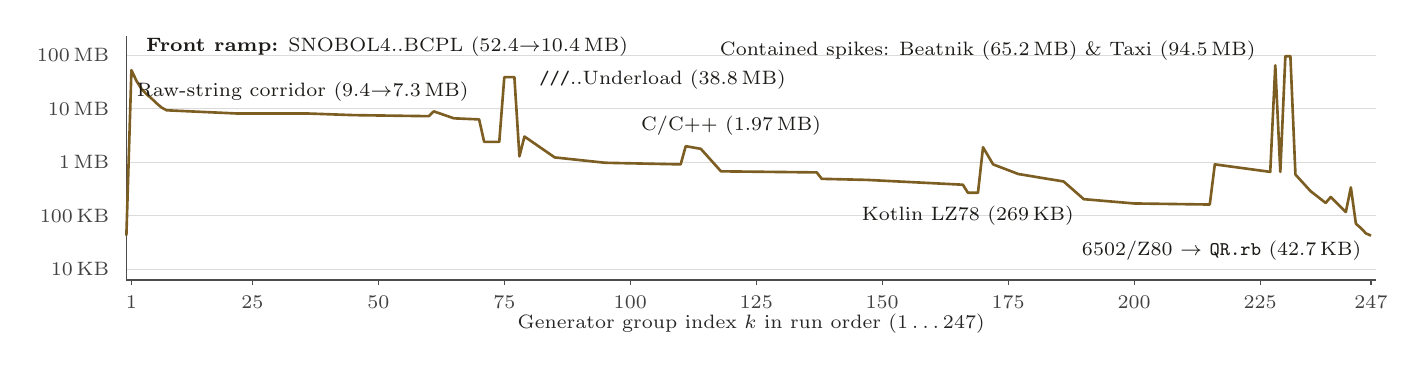
\begin{tikzpicture}[x=0.064cm,y=0.68cm]
  % Grid lines (log10 bytes: 4=10KB, 5=100KB, 6=1MB, 7=10MB, 8=100MB)
  \foreach \y/\lbl in {4/10\,KB, 5/100\,KB, 6/1\,MB, 7/10\,MB, 8/100\,MB} {
    \draw[gray!28,very thin] (0,\y) -- (248,\y);
    \node[anchor=east,font=\scriptsize,text=black!75] at (-1.5,\y) {\lbl};
  }
  \draw[black!70] (0,3.8) -- (248,3.8);
  \draw[black!70] (0,3.8) -- (0,8.35);
  \foreach \x in {1,25,50,75,100,125,150,175,200,225,247} {
    \draw[black!70] (\x,3.8) -- (\x,3.70);
    \node[anchor=north,font=\scriptsize,text=black!75] at (\x,3.68) {\x};
  }
  \node[font=\scriptsize,text=black!85] at (124,2.98) {Generator group index $k$ in run order ($1 \dots 247$)};

  % Empirical log10(bytes) trajectory from proof/zones.csv
  \draw[brass!90!black,line width=0.95pt,line join=round]
    (0,4.63) -- (1,7.72) -- (2,7.52) -- (3,7.37) -- (4,7.27) -- (5,7.19) -- (6,7.10) -- (7,7.02)
    -- (8,6.97) -- (22,6.91) -- (36,6.91) -- (45,6.88) -- (60,6.86) -- (61,6.95) -- (65,6.82)
    -- (70,6.80) -- (71,6.38) -- (74,6.38) -- (75,7.59) -- (77,7.59) -- (78,6.11) -- (79,6.48)
    -- (85,6.09) -- (95,5.99) -- (110,5.96) -- (111,6.30) -- (114,6.25) -- (118,5.83)
    -- (137,5.81) -- (138,5.69) -- (147,5.67) -- (166,5.58) -- (167,5.43) -- (169,5.43)
    -- (170,6.28) -- (172,5.96) -- (177,5.78) -- (186,5.64) -- (190,5.31) -- (200,5.23)
    -- (215,5.21) -- (216,5.96) -- (227,5.82) -- (228,7.81) -- (229,5.82) -- (230,7.98)
    -- (231,7.98) -- (232,5.77) -- (235,5.46) -- (238,5.24) -- (239,5.35) -- (242,5.07)
    -- (243,5.53) -- (244,4.85) -- (245,4.77) -- (246,4.67) -- (247,4.63);

  % Clean non-overlapping callouts across wide two-column span
  \node[font=\scriptsize,anchor=west,text=ink] at (2,8.16) {\textbf{Front ramp:} SNOBOL4..BCPL (52.4$\to$10.4\,MB)};
  \node[font=\scriptsize,anchor=south,text=ink] at (35,6.96) {Raw-string corridor (9.4$\to$7.3\,MB)};
  \node[font=\scriptsize,anchor=west,text=ink] at (80,7.55) {\texttt{///}..Underload (38.8\,MB)};
  \node[font=\scriptsize,anchor=south,text=ink] at (120,6.32) {C/C++ (1.97\,MB)};
  \node[font=\scriptsize,anchor=north,text=ink] at (167,5.37) {Kotlin LZ78 (269\,KB)};
  \node[font=\scriptsize,anchor=east,text=ink] at (226,8.08) {Contained spikes: Beatnik (65.2\,MB) \& Taxi (94.5\,MB)};
  \node[font=\scriptsize,anchor=east,text=ink] at (247,4.35) {6502/Z80 $\to$ \texttt{QR.rb} (42.7\,KB)};
\end{tikzpicture}
\vspace{-0.4em}
\caption{Log-scale intermediate payload profile ($\log_{10} L_k$) across all 247 generator groups of \texttt{quine-relay-284} (\texttt{proof/zones.csv}, group sum $1.14\text{ GB}$). Contained generator--consumer pairs isolate esolang spikes while five internal compressors step the baseline down to the 42,680-byte Ruby seed.}
\label{fig:profile}
\end{figure*}

\begin{theorem}[Front-Heavy Ratio Ordering]
\label{thm:order}
For two adjacent fixed-ratio steps $x, y$ wrapping payload $L > 0$, the outer peak $x(yL) = y(xL)$ is permutation-invariant, whereas placing the larger ratio closer to the seed ($x > y$) strictly minimizes total bytes written: $xyL + yL < yxL + xL$.
\end{theorem}
\begin{proof}
Subtracting $xyL = yxL$ from both sides reduces the inequality to $yL < xL$, which holds for all $x > y$ and $L > 0$ (\texttt{swap\_front\_heavy\_minimizes\_sum}). By adjacent-transposition induction, sorting fixed-ratio steps in non-increasing order from the front minimizes $\sum_k L_k$.
\end{proof}

Moreover, by Theorem~\ref{thm:eigen}, if $E$ escaping steps sit near the front, each special character (\texttt{\textbackslash} or \texttt{"}) emitted by an interior step $k$ costs at least $2^E$ bytes at the front. Hence our main 53-step corridor (\texttt{K}..\texttt{Scheme}, \texttt{9.41} $\to$ \texttt{7.30 MB}) uses raw/heredoc strings exclusively: 47 of 247 group outputs contain \textbf{zero} backslashes, and 110 contain fewer than 100.

\section{Overcoming Compiler, VM, and Hardware Ceilings}
\label{sec:ceilings}

Table~\ref{tab:ceilings} summarizes the principal architectural barriers encountered between 157 and 284 steps and their exact remedies.

\begin{table}[t]
\centering
\caption{Hard compiler, VM, and OS limits defeated in \texttt{quine-relay-284}.}
\label{tab:ceilings}
\vspace{2pt}
\resizebox{\columnwidth}{!}{%
\begin{tabular}{@{}p{0.84in}p{0.94in}p{1.56in}@{}}
\toprule
\textbf{Subsystem} & \textbf{Hard Ceiling} & \textbf{Architectural Solution} \\
\midrule
6502 / Z80 ISAs & $2^{16} = 65{,}536$\,B ROM & Interleaved Re-Pair assemblers (\texttt{QR.o65} = 45.1\,KB; \texttt{QR.z80.bin} = 32.0\,KB) \\
JVM (12 langs)  & $65{,}535$\,B \texttt{Utf8} & Chunked string arrays \& split methods (\texttt{m0..mN}) across Java, Clojure, Frege, Gosu \\
WebAssembly     & 2-byte LEB128 (16\,KB) & Dynamic 4-byte unsigned LEB128 ($2^{28}-1 = 256$\,MiB data segments) \\
Node / JSFuck   & V8 \texttt{Zone::Expand} & 3-digit base-78 LZ78 in Kotlin ($78^3 = 474{,}552$ codes; \texttt{QR.kt} = 269\,KB; \texttt{QR.jsfuck} = 22.3\,MB) \\
Basser Lout     & \texttt{SHORT\_MAX} $32{,}767$ & Paginated into 40-line \texttt{@NP} pages so galley height stays in 16-bit \texttt{short} \\
PAKCS (\texttt{Curry}) & SWI-Prolog $\sim$903\,KB & Compact \texttt{\textasciitilde}-escaped \texttt{Glass} + \texttt{i<"..."} \texttt{Kipple} ($15\times$ shrink; \texttt{QR.curry} = 645\,KB) \\
GNU \texttt{Makefile} & \texttt{MAX\_ARG} 128\,KB & In-process \texttt{\$\{file >QR\_m,\dots\}} write, bypassing \texttt{execve} \texttt{E2BIG} \\
\texttt{Shakespeare} & \texttt{spl2c}/\texttt{gcc} $>150$\,MB & $O(1)$-AST 50.2\,KB play emitting 401\,B \texttt{S-Lang} decoder reading \texttt{QR.sci} \\
\texttt{Hexagony} & Hex grid corner rule & Zero-backslash \texttt{<}/\texttt{/}/\texttt{>} boustrophedon snake on \texttt{m-ender/hexagony} \\
\bottomrule
\end{tabular}%
}
\end{table}

\paragraph{1. $O(1)$-AST Self-Reading Comment Decoders.}
Compiling a naive literal-printing program $P_k$ requires parsing $\Theta(|P_{k+1}|)$ AST nodes, which stalls legacy or theatrical compilers (\texttt{spl2c} on \texttt{Shakespeare}, \texttt{CSNOBOL4}, \texttt{GNU Cim} \texttt{Simula}, \texttt{OBNC} \texttt{Oberon}, \texttt{GNU MARST} \texttt{ALGOL 60}, \texttt{BCPL}). Decomposing $P_k = D_k \mathbin{\|} C_k(P_{k+1})$ into a constant-size self-reading decoder $D_k$ ($|D_k| = 200\text{--}600\text{ B}$) that opens its own source file and decodes lexer-inert comment lines $C_k$ decouples compiler AST complexity from payload size ($\Theta(1)$ parse tree, $\Theta(|P_{k+1}|)$ linear I/O) with zero external data files.

\paragraph{2. Interleaved Re-Pair Assembly Compression (Theorem 4).}
Literal byte-directive assemblers (\texttt{.byte 34,\dots}) expand payloads by $\alpha \ge 3\times$; two consecutive literal assemblers satisfy $3(3x + b_1) + b_2 > 65{,}536$ whenever $x \ge 7{,}282\text{ B}$ (\texttt{adjacent\_litAsm\_overflows\_64k}). By alternating pair-dictionary decompressing assemblers with literal assemblers across six architectures (\texttt{Uxntal} $\to$ \texttt{MMIX} $\to$ \texttt{6502} $\to$ \texttt{ARM64} $\to$ \texttt{Z80} $\to$ \texttt{RISC-V}), each contractive--expansive pair satisfies $\text{pair}(y) \le M$, keeping assembled 8-bit binaries well inside 64\,KB (\texttt{QR.o65} $= 45{,}083\text{ B}$, \texttt{QR.z80.bin} $= 32{,}039\text{ B}$).

\paragraph{3. Base-78 3-Digit LZ78 Dictionary Scaling (Theorem 5).}
\texttt{Kotlin} compresses \texttt{TXR} (\texttt{1.91 MB}) ahead of \texttt{JavaScript $\to$ jq $\to$ JSFuck}. Drawing safe printable ASCII digits from the 84-byte window \texttt{42..125} (excluding 6 characters for radix $78$), 2-digit codes ($78^2 = 6{,}084$) saturate prematurely, whereas 3-digit codes (\texttt{q*78}, \texttt{/6084}) yield $78^3 = 474{,}552$ codewords---exact capacity for our $474{,}551 = 78^3 - 1$ dictionary cap (\texttt{base78\_lz78\_capacity\_exact}), compressing \texttt{QR.kt} to \texttt{269 KB} and keeping \texttt{QR.jsfuck} at \texttt{22,340,708 B} (\texttt{22.3 MB}, $\sim$5\,s in V8).

\section{Metaprogramming Soundness and Formal Verification}
\label{sec:formal}

\paragraph{The \texttt{ABBREV} Pre-Escape Hazard.}
Endoh's seed generator (\texttt{src/QR.rb.gen.rb}) concatenates all step generators into a single Ruby expression $s$, globally hex-escapes every byte in $K = \text{dom}(\texttt{ABBREV})$ (\texttt{\textasciitilde}, \texttt{`}, \texttt{K}, \texttt{J}, \texttt{Y}, \texttt{H}, \texttt{\textasciicircum}, \texttt{X}, \texttt{Z}, \texttt{G}, \texttt{U}, \texttt{!}) via $b \mapsto \texttt{\textbackslash xHH}$, substitutes single-byte macro keys from $K$, and wraps the result in \texttt{eval\$s=\%q(\dots)} with runtime \texttt{.tr} expansion. During development, an inner generator containing Ruby's regex-match operator \texttt{b20c =\textasciitilde{} /\dots/} was transformed by pre-escaping into \texttt{b20c =\textbackslash x7e /\dots/}, causing a \texttt{SyntaxError} on Step~1!

In \texttt{proof/formal/}, we model Ruby token contexts over \texttt{StrLit}$(bs)$ (\texttt{"..."}), \texttt{RawLit}$(bs)$ (\texttt{\%q(...)}), and \texttt{OpTok}$(bs)$ (operators and syntax), proving both the corruption witness $\texttt{evalEscapedTok}(\{\texttt{0x7e}\},\allowbreak \texttt{OpTok}[\texttt{0x3d},\texttt{0x7e}]) = \texttt{none}$ and the exact non-interference theorem: \emph{pre-escaping is an exact semantic identity across all tokens if and only if \texttt{RawLit} and \texttt{OpTok} tokens are disjoint from $K$} (\texttt{abbrev\_safe\_token\_identity}).

\paragraph{Dual-Kernel Machine-Checked Proofs.}
All seven theorem suites---(1)~$\Phi/\Psi$ affine escape dynamics, (2)~zero-residual delimiter reset, (3)~front-heavy ratio ordering, (4)~64\,KB interleaved assembly invariant, (5)~base-78 LZ78 capacity, (6)~\texttt{ABBREV} token soundness, and (7)~$N$-step Uroboros cycle closure ($[\![ P_1 ]\!]_{1..N} = P_1$)---were formalized independently in \textbf{Lean~4.35.0} (\texttt{QuineRelayTheorems.lean}, 296 lines, \texttt{0 sorry}) and \textbf{Rocq~8.20.1} (\texttt{QuineRelayTheorems.v}, 292 lines, verified by \texttt{coqchk -silent -o QuineRelayTheorems} with \texttt{Axioms: <none>}). Notably, interactive formalization actively improved the paper: Lean~4's \texttt{omega} solver falsified a hand-derived $+(2^{k+1}-4)$ remainder in Theorem~\ref{thm:reset} to reveal exact cancellation, and Rocq's \texttt{lia} caught a ones-digit arithmetic slip ($170{,}307{,}648 \to 170{,}307{,}272$).

\section{Empirical Evaluation and Independent Audit}
\label{sec:eval}

Table~\ref{tab:compare} compares \texttt{quine-relay-284} against upstream \texttt{mame/quine-relay} (\texttt{900c941}) and \texttt{quine-relay-151}, alongside intra-group intermediate files measured directly inside the \texttt{qr284} container.

\begin{table}[t]
\centering
\caption{End-to-end comparison across verified Uroboros relays on Ubuntu 26.04.}
\label{tab:compare}
\vspace{2pt}
\resizebox{\columnwidth}{!}{%
\begin{tabular}{@{}lrrr@{}}
\toprule
\textbf{Metric} & \textbf{\texttt{mame} (128)} & \textbf{Relay 151} & \textbf{Relay 284} \\
\midrule
Tier-1 distinct languages & 123 & 143 & \textbf{273} \\
Tier-2 relay steps ($\le 3$/fam.) & 128 & 151 & \textbf{284} \\
Retired \texttt{mame} langs restored & --- & 2 / 20 & \textbf{17 / 20} \\
Seed size (\texttt{QR.rb}) & 13,664\,B & 14,868\,B & \textbf{42,680\,B} \\
Seed bytes per step & 106.8\,B & \textbf{98.5\,B} & 150.3\,B \\
Main raw corridor & 27.9\,KB med. & $\sim$3.0\,MB & \textbf{7.30--9.41\,MB} \\
Peak group output (\texttt{zones.csv}) & 4.49\,MB (\texttt{sq}) & $\sim$3.1\,MB & \textbf{94.55\,MB} (\texttt{Taxi}) \\
Intra-group (\texttt{sq} / \texttt{ook}) & 4.49 / 4.69\,MB & $\sim$4.7\,MB & \textbf{58.10 / 48.77\,MB} \\
Other intra (\texttt{jsfuck}/\texttt{mid}/\texttt{spl}) & --- & --- & \textbf{22.3 / 12.1 / 0.05\,MB} \\
Total group bytes per lap & 50.89\,MB & $\sim$180\,MB & \textbf{1.14\,GB} \\
Clean \texttt{--no-cache} build & $\sim$8\,min & $\sim$14\,min & \textbf{4,189\,s} (69m\,49s) \\
Full verification lap & 474\,s & $\sim$720\,s & \textbf{2,377\,s} (39m\,37s) \\
Closure (\texttt{diff QR.rb QR2.rb}) & Identical & Identical & \textbf{Identical} \\
\bottomrule
\end{tabular}%
}
\end{table}

\paragraph{Independent Upstream Interpreter \& CPU Audit.}
To rule out permissive shortcuts in bundled interpreters (\texttt{audit/AUDIT.md}), all five custom esolang transitions and both 8-bit CPU steps were extracted at full 284-step payload scale and executed on canonical upstream/third-party implementations:
\begin{enumerate}
  \item \textbf{Hexagony (\#77):} Martin B\"uttner's \texttt{m-ender/hexagony} (\texttt{b674f59}) $\to$ \texttt{2,375,282\,B} (\textbf{exact SHA-256 match}).
  \item \textbf{Emmental (\#126):} Chris Pressey's Haskell \texttt{catseye/Emmental} $\to$ \texttt{1,772,824\,B} (\textbf{exact match}).
  \item \textbf{Rail (\#255):} Jonathon Duerig's C++ \texttt{TryItOnline/rail} (\texttt{04b7259}, \texttt{\$ 'main'}) $\to$ \texttt{665,576\,B} (\textbf{exact match}).
  \item \textbf{Kipple (\#256):} Jannis Harder's \texttt{cipple 0.2.1} \& Rune Berge's \texttt{Kipple.jar} $\to$ \texttt{65,234,873\,B} (\textbf{exact match}).
  \item \textbf{Glass (\#258):} Gregor Richards' \texttt{glass-0.12} C++ \& \texttt{vendor/glass.rb} $\to$ \texttt{94,546,636\,B} (\textbf{exact match}).
  \item \textbf{MOS 6502 (\#268) \& Zilog Z80 (\#270):} Mike Naberezny's \texttt{py65 1.2.0} (\texttt{45,083 B} $\to$ \texttt{149,485 B}) and \texttt{z80 1.2.0} C core (\texttt{32,039 B} $\to$ \texttt{339,973 B}) $\to$ \textbf{exact SHA-256 matches}.
\end{enumerate}

\section{Reproducibility}

All source generators, Dockerfiles, formal proof scripts, and complete build/run logs are MIT-licensed at \url{https://github.com/exacortex/quine-relay-284}:
\begin{lstlisting}
git clone https://github.com/exacortex/quine-relay-284 && cd quine-relay-284
docker build --no-cache -t qr284 . && docker run --rm qr284
python3 tools/verify_invariants.py
\end{lstlisting}

\footnotesize
\begin{thebibliography}{9}
\setlength{\itemsep}{1pt}
\setlength{\parskip}{0pt}
\bibitem{kleene1938}
S.~C. Kleene, ``On notation for ordinal numbers,'' \emph{Journal of Symbolic Logic}, vol.~3, no.~4, pp.~150--155, 1938.
\bibitem{endoh2018}
Y.~Endoh (\texttt{@mametter}), ``Quine Relay: An uroboros program with 100+ programming languages,'' GitHub repository \url{https://github.com/mame/quine-relay}, 2013--2026.
\bibitem{larsson1999}
N.~J. Larsson and A.~Moffat, ``Offline dictionary-based compression (Re-Pair),'' \emph{Proc.\ IEEE Data Compression Conf.\ (DCC)}, pp.~296--305, 1999.
\bibitem{ziv1978}
J.~Ziv and A.~Lempel, ``Compression of individual sequences via variable-rate coding,'' \emph{IEEE Trans.\ Inf.\ Theory}, vol.~24, no.~5, pp.~530--536, 1978.
\bibitem{moura2021}
L.~de Moura and S.~Ullrich, ``The Lean 4 theorem prover and programming language,'' \emph{Proc.\ CADE-28}, LNCS 12699, pp.~625--635, 2021.
\bibitem{coq2024}
The Coq Development Team, \emph{The Coq / Rocq Proof Assistant Reference Manual, Version 8.20}, INRIA, 2024.
\end{thebibliography}

\end{document}
